\chapter{Computational results}\label{ch:computational-results}

This chapter presents the computational results of the proposed solution,
generated dataset, hyperparameters of the genetic algorithm,
and implementation of the computation server
to which a user can submit a painting placement instance and receive a solution to that instance.

First, four testing scenarios used for evaluation are described in
section~\ref{sec:scenarios}.
They are random, clustering, packing, and London National Gallery.
Next, in section~\ref{sec:dataset}, the dataset created for each testing scenario is described.
Then, section~\ref{sec:hyper-parameters} describes and discusses
the hyperparameters of the proposed genetic algorithm~\ref{alg:genetic}.
Also, reasonable hyperparameter values are determined.
Section~\ref{sec:results} presents a painting placement solutions to the painting placement instances and their visualizations.
Lastly, section~\ref{sec:implementation} describes the implementation of the computation server.

\section{Scenarios}\label{sec:scenarios}

Four testing scenarios evaluate different aspects of the proposed solution.
They are random, clustering, and packing.
Additionally, one scenario describes the painting placement at the London National Gallery in figure~\ref{fig:london-wall}. \\

\navesti{Random} scenario contains randomly generated painting placement instances.
It is mainly used for performance testing.
\\

\navesti{Clustering} scenario tests the ability to form clusters.
It is achieved by dividing the paintings into groups.
Paintings belonging to the same group have increased flow between them.
Paintings from the distinct group have flow between them set to 0.
\\

\navesti{Packing} scenario is the same as the random scenario, with the only difference being that the layout area is equal to the area of all paintings summed together.
It tests the ability to create compact solutions.
\\



\section{Dataset}\label{sec:dataset}

This section describes the parameters used to create datasets for each testing scenario in subsection~\ref{subsec:generation-parameters}.
Generated instances are described in subsection~\ref{subsec:instances}.

Additionally, as mentioned in chapter~\ref{ch:literature-review}, no datasets in the
literature would satisfy the definition~\ref{eq:painting-placement-instance} of painting placement instance.
Thus, all datasets are exclusively created by the author and can be used by other researchers
for benchmarking their solutions.

Generation of testing instances is performed using a Python programming language in combination with Jupyter Notebook.
Both the datasets and Notebooks are in the attached medium.

\subsection{Generation parameters}\label{subsec:generation-parameters}

Seven parameters are used for dataset generation.
They are layout area ratio, max painting ratio, eval function, max painting width, max painting height, flow min, and flow max.
Their values for generating instances for testing scenarios are in table~\ref{tab:generation-parameters}.
A description of each of them follows in the rest of this subsection.

\begin{table}[h!]
    \caption{Parameters used to generate testing scenarios}
    \begin{threeparttable}
        \begin{tabular}{llllllll}
            \hline
            \textbf{Scenario} &
            \textbf{\begin{tabular}[c]{@{}l@{}}
                        Layout\\ area ratio
            \end{tabular}} &
            \textbf{\begin{tabular}[c]{@{}l@{}}
                        Max paint.\\ width
            \end{tabular}} &
            \textbf{\begin{tabular}[c]{@{}l@{}}
                        Max paint.\\ height
            \end{tabular}} &
            \textbf{\begin{tabular}[c]{@{}l@{}}
                        Max paint.\\ ratio
            \end{tabular}} &
            \textbf{\begin{tabular}[c]{@{}l@{}}
                        Flow\\ min
            \end{tabular}} &
            \textbf{\begin{tabular}[c]{@{}l@{}}
                        Flow\\ max
            \end{tabular}} &
            \textbf{\begin{tabular}[c]{@{}l@{}}
                        Eval\\ function
            \end{tabular}}  \\ \hline
            random & 1.2 & 10 & 10 & 3 & 0 & 4 & $f(x,y) = x+y$   \\ \hline
            cluster & 1.2   & 10 & 10 & 3 & - & - & $f(x,y) = 0$   \\ \hline
            packing & 1 & 10 & 10 & 3 & 0 & 4 & $f(x,y) = 0$ \\ \hline
            \begin{tabular}[c]{@{}l@{}}
                biased\\ clustering
            \end{tabular} & 1.3 & 10 & 10 & 3 & - & - & - \\ \hline
        \end{tabular}
        \begin{tablenotes}
            \small
            \item Left-out values marked with - are discussed later in the text.
        \end{tablenotes}
    \end{threeparttable}
    \label{tab:generation-parameters}
\end{table}

\definice{Layout area ratio} is the ratio between the area of the layout and the painting area sum.
It is computed as

\[
    \dfrac{\sum\limits_{i=1}^{N} w_i h_i}{WH}\,,
\]

where $w_i$ is width, $h_i$ is height of painting $i$, $W$ is width, and $H$ is height of the layout.
If the layout area ratio is set to $1$, it means a preference for more compact layouts.
On the other hand,
increasing this value implies the presence of more free space in the resulting layout.

\definice{Max painting ratio} controls the maximum aspect ratio between width $w$ and height $h$ of each painting.
It is computed as

\[
    \dfrac{\max(w,h)}{\min(w,h)}\,.
\]

Increasing the max painting ratio implies the possibility of the generation of paintings
that are very thin, i.e., $w \ll h$ or $h \ll w$.
On the other hand, setting the value to 1
implies that every generated painting is square.

\definice{Eval function} is function $\pi$ from eq.~\ref{eq:objective}.
In the random scenario, the eval function is set to $f(x,y) = x+y$ because of its simplicity, linearity, and interpretability.
Also, it implies that it is advantageous to place small paintings close to the bottom left corner as the function value is the lowest there and
big paintings to the top right corner.
On the other hand, for clustering and packing scenarios, the eval function is set to a constant value $f(x,y) = 0$.
The reason is that different capabilities are tested (clustering and packing).
Furthermore, using a non-constant eval function makes it harder to interpret the results.

Rest of the parameters, \definice{max painting width}, \definice{max painting height}, \definice{flow min}, \definice{flow max}
are self-explanatory and were set as low numeric values to increase computation speed and avoid overflow.

\subsection{Instances}\label{subsec:instances}

Seven painting placement instances are generated using table~\ref{tab:generation-parameters} parameters.
Generated instances are described in table~\ref{tab:instances}.
For random and packing scenarios, values for max painting width/height, flow min/max, and max painting ratio are randomly generated from the parameter range described in table~\ref{tab:generation-parameters}.
The clustering and biased clustering parameters are also generated randomly.
The only exception is the flow, which is set in a way to form clusters.

Visualization of the flow for two painting placement instances is in appendix in figure~\ref{fig:instance-flow}.
On the left is the randomly generated flow for random\_10 instance, and on the right is the flow for cluster\_3\_6 instance that forms clusters.

Lastly, the eval function for biased\_sparse\_cluster\_3\_5 partitions the layout into six same-size chessboard squares.
Half are assigned the same advantageous evaluation to force the cluster formation.
The second half is evaluated to zero.
The concrete value for the eval function is in the appendix in listing~\ref{lst:biased-sparse-cluster-eval-function}.

\begin{table}[h!]
    \caption{Values of generated instances}
    \label{tab:instances}
    \begin{tabular}{lllll}
        \hline
        \textbf{Instance name} &
        \textbf{\begin{tabular}[c]{@{}l@{}}
                    Paint.\\ count
        \end{tabular}} &
        \textbf{\begin{tabular}[c]{@{}l@{}}
                    Layout\\ width, height
        \end{tabular}} &
        \textbf{Scenario} &
        \textbf{Description} \\ \hline
        random\_10    & 10 & 24 x 19 & random     &                                        \\ \hline
        random\_20    & 20 & 31 x 25 & random     &                                        \\ \hline
        packing\_10   & 10 & 19 x 15 & packing    &                                        \\ \hline
        packing\_20   & 20 & 33 x 26 & packing    &                                        \\ \hline
        cluster\_3\_6 & 18 & 30 x 25 & clustering & \begin{tabular}[c]{@{}l@{}}
                                                        3 clusters,\\ 6 paintings each
        \end{tabular} \\ \hline
        cluster\_4\_5 & 20 & 34 x 27 & clustering & \begin{tabular}[c]{@{}l@{}}
                                                        4 clusters,\\ 5 paintings each
        \end{tabular} \\ \hline
        biased\_sparse\_cluster\_3\_5 &
        15 &
        29 x 23 &
        biased clustering &
        \begin{tabular}[c]{@{}l@{}}
            3 clusters,\\ 5 paintings each
        \end{tabular} \\ \hline
    \end{tabular}
\end{table}}




\newpage


\section{Hyper-parameters}\label{sec:hyper-parameters}

There are eight hyperparameters to the proposed genetic algorithm~\ref{alg:genetic}.
They are described in table~\ref{tab:hyperparams}.
An example of these hyperparameter values is in listing~\ref{lst:computation-submission-dataset}.
The rest of the sections discuss these hyperparameters further and tries to find their reasonable values.

\subsection{Max number of iter}\label{subsec:max-number-of-iter}
Results for hyperparameter \verb|maxNumberOfIter| are in figure~\ref{fig:hyperparams-max-number-of-iter}.
We can see the initial decrease of the average population objective for both random instances.
Between iterations 100 and 150, decreasing trend and fluctuations stop.
From it, we can deduce that at least 150 iterations are needed.

\subsection{Population size}\label{subsec:population-size}

Population size is calculated as $kN$, where $k$ is \definice{population scaling factor}
and $N$ is instance size.
Thus, the population size is linear with respect to the instance size.

Results for two random instances are in figure~\ref{fig:hyperparameters-population-size}.
We can see that scaling factor $10$ does not allow
the population objective average to decrease to the levels comparable to scaling factors $50$ and $100$.
It might imply that the scaling factor $10$ cannot represent knowledge gathered over time
in the genetic algorithm or that more iterations are needed.

The conclusion is that using scaling factor between $50$ and $100$ is sufficient, with bias towards $100$
for obtaining better average objective performance.
However, increasing the scaling factor leads to slower computation speed as every population contains
more individuals for which genetic operators and reproductive plan must be computed.

\subsection{Maximum wild card count}\label{subsec:maximum-wild-card-count}
Hyperparameter \verb|maximumWildCardCount| limits the maximum number of $*$ cut types produced by $OR_{prob}$ decoding.
It is recommended to keep this hyperparameter very low or even set it to zero.
The reason is that if it is high, computation time increases as $*$ spreads in the population.
For example, consider an individual whose orientation vector is solely composed of $*$ cut types.
If the size of that vector is $n$, individual decodes to $2^n$ resolved slicing trees as seen in figure~\ref{fig:layout-construction-steps}.

\subsection{Orientation weights}\label{subsec:orientation-weights}
TODO

\subsection{Population division counts}\label{subsec:population-division-counts}
TODO

\subsection{Initial population division counts}\label{subsec:initial-population-division-counts}
TODO

\subsection{Overlapping penalization constant}\label{subsec:overlapping-penalization-constant}

It is not desirable to produce painting placement solutions that overlap.
Thus, hyperparameter \verb|overlappingPenalizationConstant| penalizes
individuals representing such a solution.

The optimal value must be strong enough to remove or limit overlapping solutions from the population.
Also, it must be low enough not to become the dominant part of the objective function (eq.~\ref{eq:objective})
as it can lead the genetic algorithm to neglect other parts – eval function, clustering, and flow between paintings.

Values tested for \verb|overlappingPenalizationConstant| are proportional to the diagonal
length of the layout to which paintings are placed.
It means that if we define constant $k$, width of the layout as $W$ and its height as $H$,
tested value is $k\sqrt{W^2 + H^2}$.

Results are in figure~\ref{fig:overlapping-penalization} for two instances.
From it, we can deduce that the optimal value for \textit{overlapping penalization constant} is between $2$ and $5$ times the length of the layout diagonal.

\subsection{Outside of allocated area penalization constant}\label{subsec:outside-of-allocated-area-penalization-constant}
TODO

\begin{landscape}% Landscape page
    \begin{table}[]
        \caption{Hyperparameters of the genetic algorithm}
        \label{tab:hyperparams}
        \begin{tabular}{lcc}
            \hline
            \textbf{hyperparameter} &
            \textbf{\begin{tabular}[c]{@{}c@{}}
                        recommended\\ value
            \end{tabular}} &
            \textbf{description} \\ \hline
            \verb|maxNumberOfIter| &
            $\ge 150$ &
            maximum number of iterations \\ \hline
            \verb|populationSize| &
            \begin{tabular}[c]{@{}c@{}}
                population scaling factor\\ \numrange{50}{100}
            \end{tabular} &
            population size \\ \hline
            \verb|maximumWildCardCount| &
            1 &
            \begin{tabular}[c]{@{}c@{}}
                limit on the maximum number of $*$ cut types\\ produced by $OR_{prob}$ decoding
            \end{tabular} \\ \hline
            \verb|orientationWeights| &
            TODO &
            penalization vector $P$ from eq.~\ref{eq:crossover-orprob} \\ \hline
            \verb|populationDivisionCounts| &
            TODO &
            \begin{tabular}[c]{@{}c@{}}
                reproductive plan ratios\\ (left part of fig.~\ref{fig:population-schema})
            \end{tabular} \\ \hline
            \verb|initialPopulationDivisionCounts| &
            TODO &
            \begin{tabular}[c]{@{}c@{}}
                initial population ratios\\ (right part of fig.~\ref{fig:population-schema})
            \end{tabular} \\ \hline
            \verb|overlappingPenalizationConstant| &
            \begin{tabular}[c]{@{}c@{}}
                diagonal length\\ of the layout
            \end{tabular} &
            \begin{tabular}[c]{@{}c@{}}
                overlapping paintings penalization\\ parameter $\lambda$ from eq.~\ref{eq:objective}
            \end{tabular} \\ \hline
            \verb|outsideOfAllocatedAreaPenalizationConstant| &
            \begin{tabular}[c]{@{}c@{}}
                diagonal length\\ of the layout
            \end{tabular} &
            \begin{tabular}[c]{@{}c@{}}
                outside of allocated area penalization\\ parameter $\gamma$ from eq.~\ref{eq:objective}
            \end{tabular} \\ \hline
        \end{tabular}
    \end{table}
\end{landscape}


%\afterpage{%
\clearpage% Flush earlier floats (otherwise order might not be correct)
%    \begin{landscape}% Landscape page
\begin{figure}
    \centering
    \subfloat{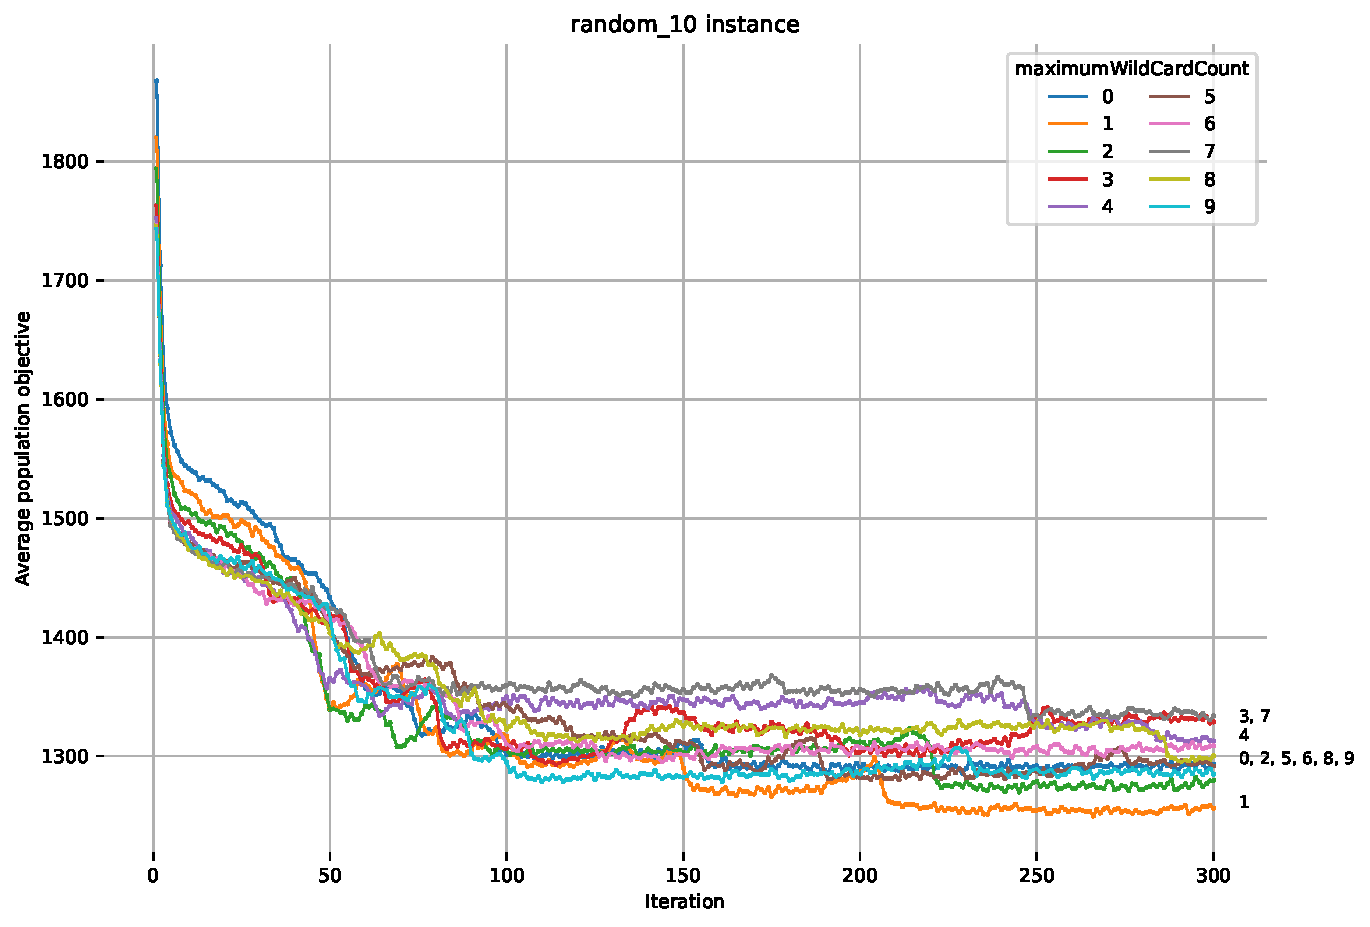
\includegraphics[width=1.1\textwidth]{hyperparameters/maximum_wild_card_count_performance_random_10}\label{subfig:hyperparams-maximum-wild-card-count-performance}}

    \subfloat{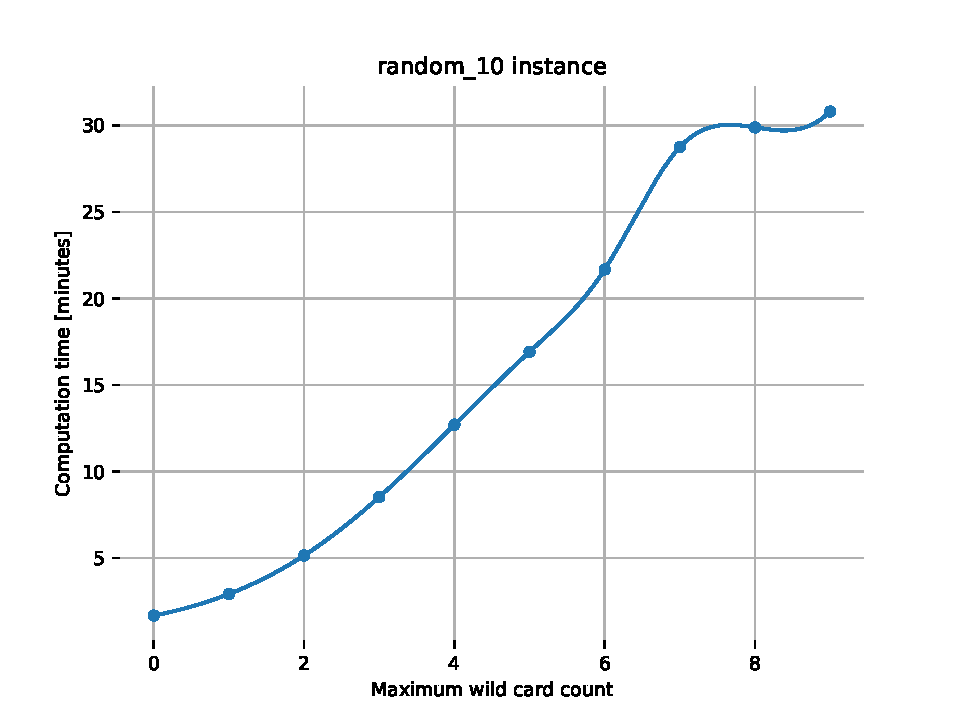
\includegraphics[width=0.8\textwidth]{hyperparameters/maximum_wild_card_count_computation_time_random_10}\label{subfig:hyperparams-maximum-wild-card-count-computation-speed}}
    \caption[Testing maximum wild card count]
    {Testing performance (top) and computation speed (bottom) for increasing maximum wild card count.}
    \label{fig:computation-time}%
\end{figure}
%    \end{landscape}
%    \clearpage% Flush page
%}

\afterpage{%
    \clearpage% Flush earlier floats (otherwise order might not be correct)
    \begin{landscape}% Landscape page
        \begin{figure}
            \centering
            \subfloat{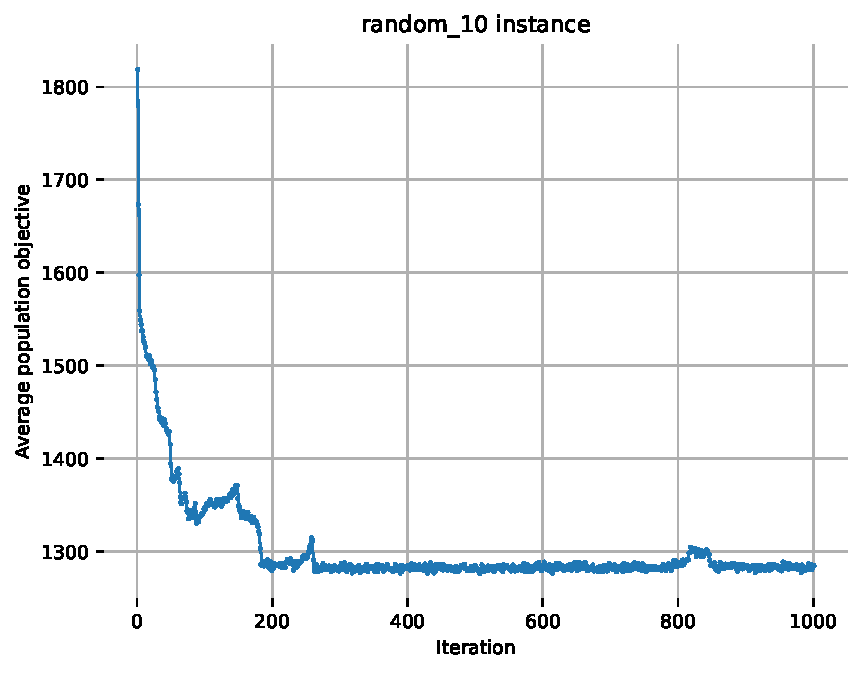
\includegraphics[width=0.8\textwidth]{hyperparameters/max_number_of_iter_random_10}\label{subfig:hyperparams-max-number-of-iter-random-10}}
            \subfloat{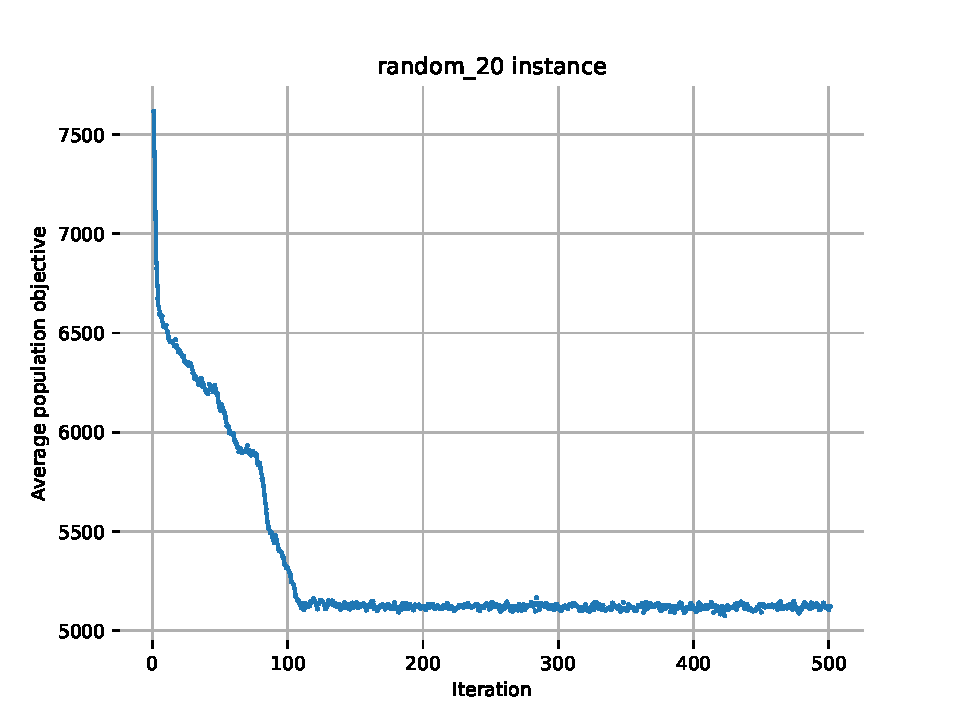
\includegraphics[width=0.8\textwidth]{hyperparameters/max_number_of_iter_random_20}\label{subfig:hyperparams-max-number-of-iter-random-20}}
            \caption[Testing maximum number of iterations]
            {Testing maximum number of iterations at two random instances.}
            \label{fig:hyperparams-max-number-of-iter}%
        \end{figure}
    \end{landscape}
    \clearpage% Flush page
}

\afterpage{%
    \clearpage% Flush earlier floats (otherwise order might not be correct)
    \begin{landscape}% Landscape page
        \begin{figure}
            \centering
            \subfloat{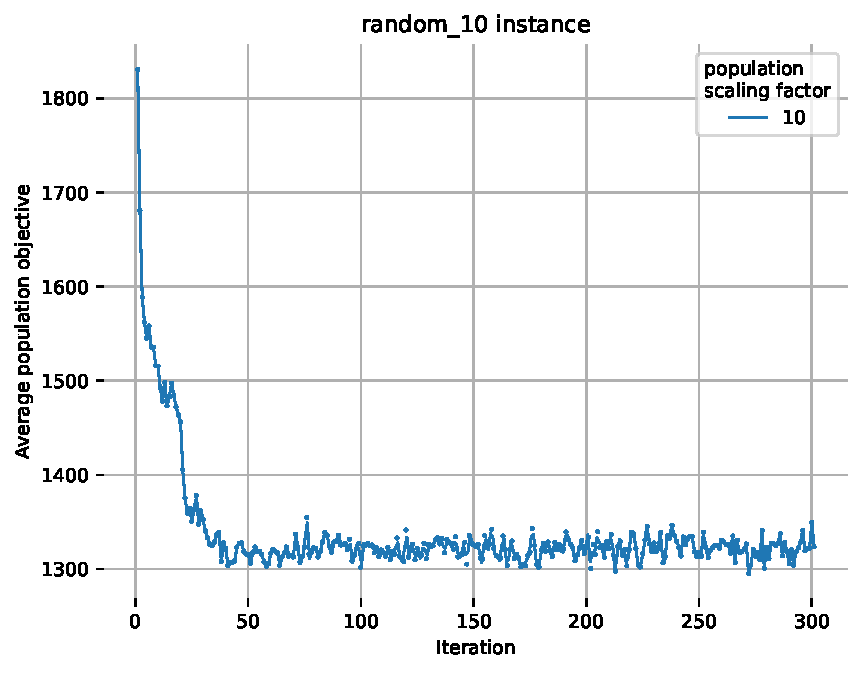
\includegraphics[width=0.8\textwidth]{hyperparameters/population_size_random_10}\label{subfig:hyperparams-population-size-random-10}}
            \subfloat{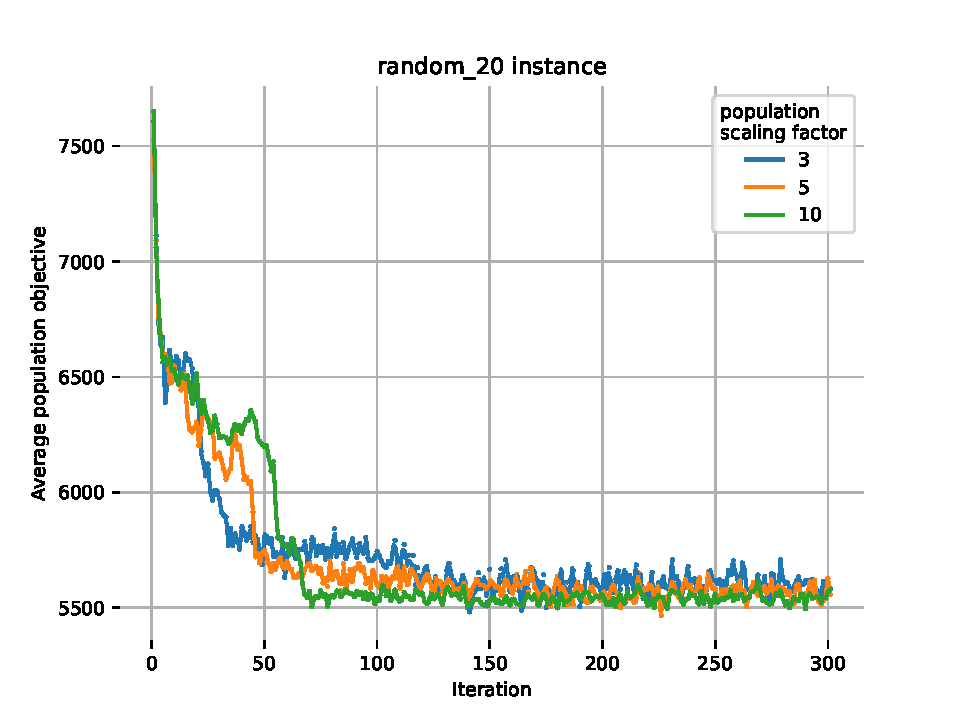
\includegraphics[width=0.8\textwidth]{hyperparameters/population_size_random_20}\label{subfig:hyperparameters-population-size-random-20}}
            \caption[Testing population scaling factor]
            {Testing population scaling factor at two random instances.
            The population size is $kN$ for population scaling factor $k$ and instance of size $N$. }
            \label{fig:hyperparameters-population-size}%
        \end{figure}
    \end{landscape}
    \clearpage% Flush page
}

\afterpage{%
    \clearpage% Flush earlier floats (otherwise order might not be correct)
    \begin{landscape}% Landscape page
        \begin{figure}
            \centering
            \subfloat{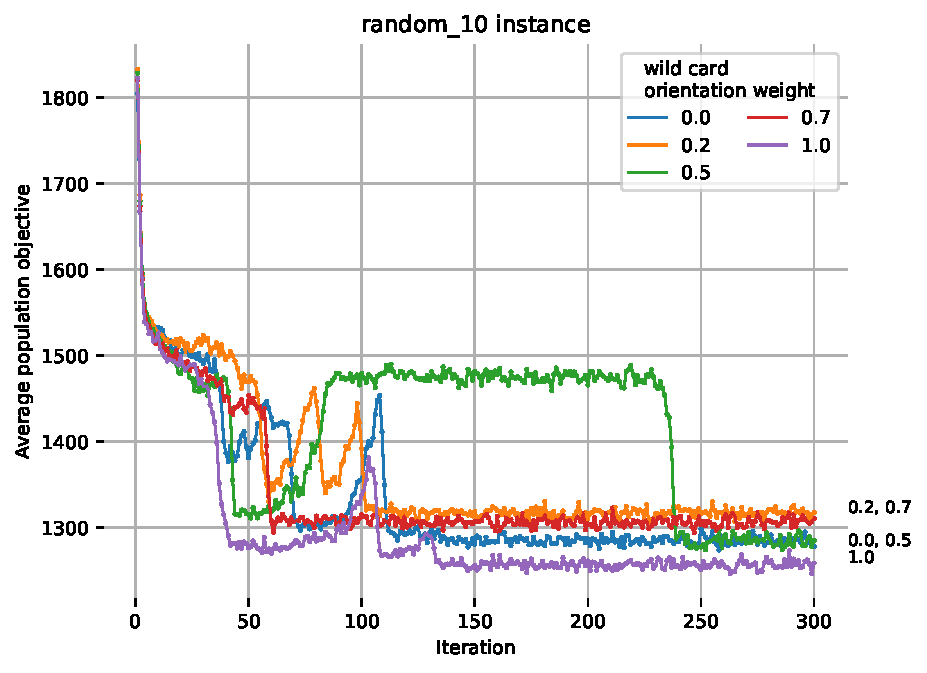
\includegraphics[width=0.8\textwidth]{hyperparameters/orientation_weights_random_10}\label{subfig:hyperparams-orientation-weights-random-10}}
            \subfloat{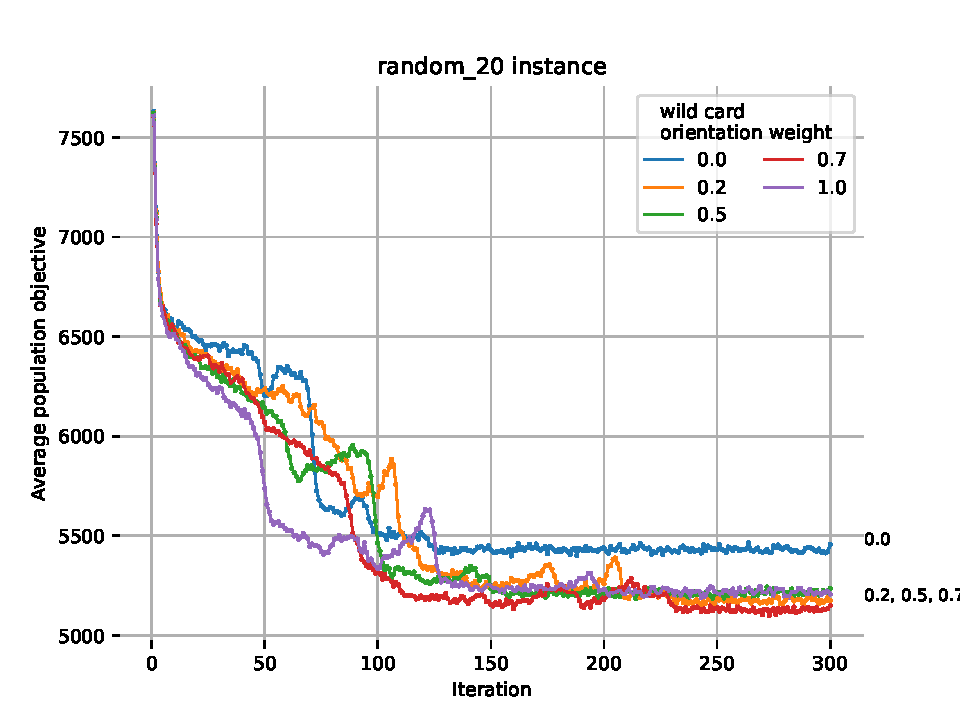
\includegraphics[width=0.8\textwidth]{hyperparameters/orientation_weights_random_20}\label{subfig:hyperparameters-orientation-weights-random-20}}
            \caption[Testing orientation weights]
            {Testing orientation weight for a wildcard cut type $*$ at two random instances.}
            \label{fig:hyperparameters-orientation-weights}%
        \end{figure}
    \end{landscape}
    \clearpage% Flush page
}

\afterpage{%
    \clearpage% Flush earlier floats (otherwise order might not be correct)
    \begin{landscape}% Landscape page
        \begin{figure}
            \centering
            \subfloat{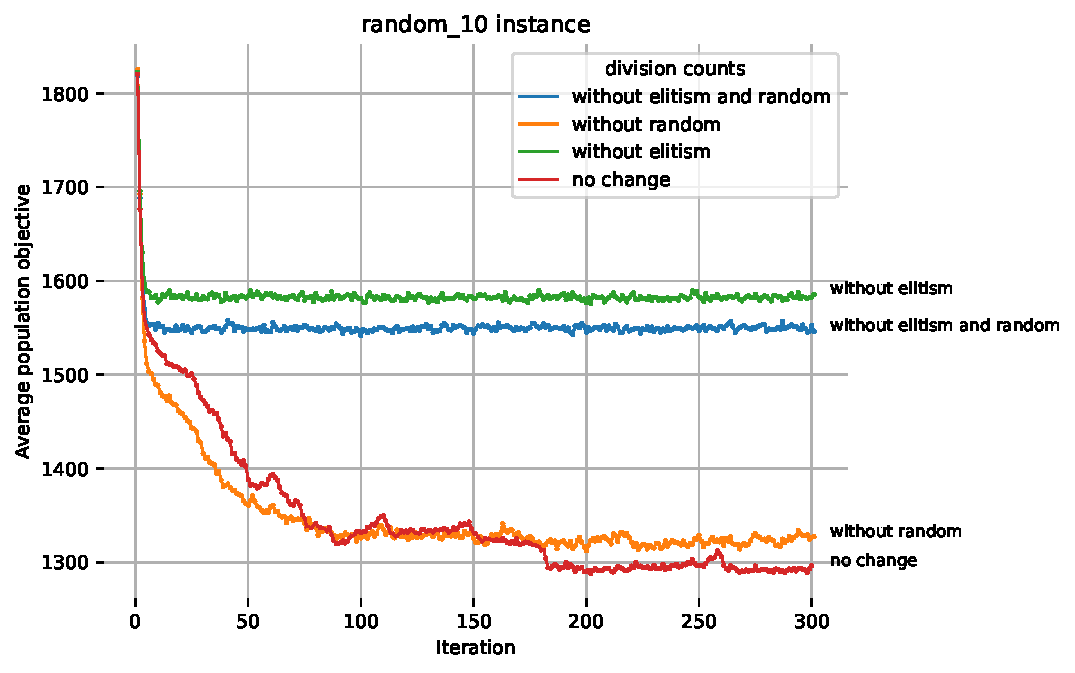
\includegraphics[width=0.8\textwidth]{hyperparameters/population_division_counts_random_10}\label{subfig:hyperparameters-population-division-counts-random-10}}
            \subfloat{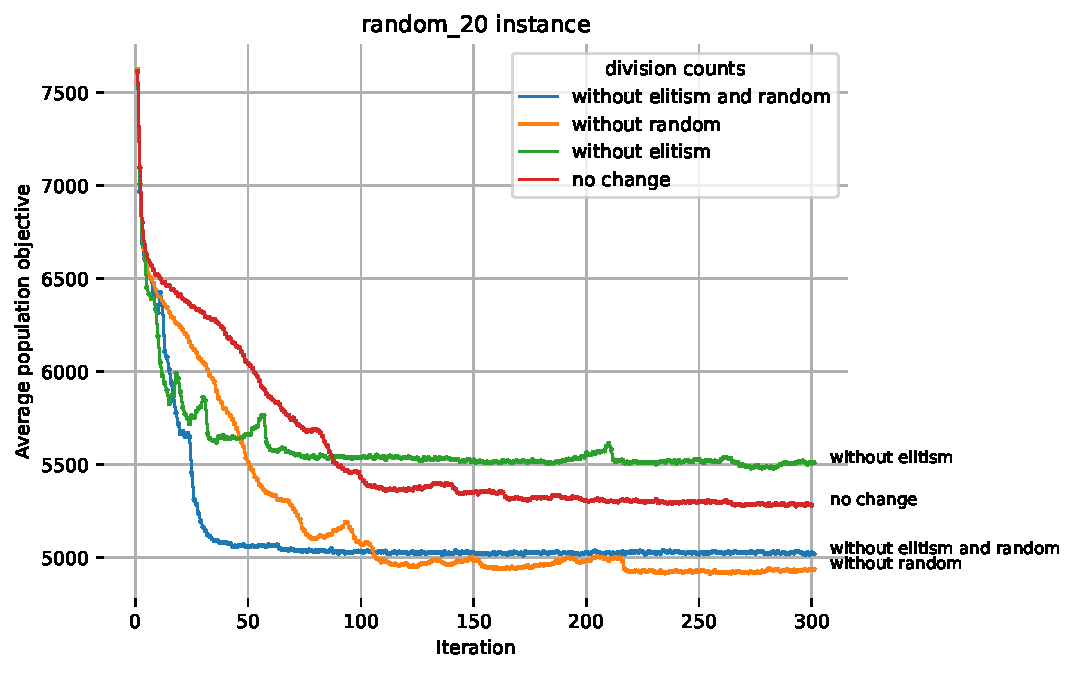
\includegraphics[width=0.8\textwidth]{hyperparameters/population_division_counts_random_20}\label{subfig:hyperparameters-population-division-counts-random-20}}
            \caption[Testing population division counts]
            {Testing population division counts at two random instances.
            Four variants are displayed. First does not use elitism, second does not inject random individuals, third combines first and second,
                and the last does not make any change to the population division counts.}
            \label{fig:hyperparameters-population-division-counts}%
        \end{figure}
    \end{landscape}
    \clearpage% Flush page
}


\clearpage% Flush earlier floats (otherwise order might not be correct)
\newpage


\section{Results}\label{sec:results}
This section presents a painting placement solution to the seven painting placement instances described in table~\ref{tab:instances}.

Hyperparameter values used to obtain all results in this section are in table~\ref{tab:hyperparameters-values}.
They are selected based on the hyperparameter testing from section~\ref{sec:hyper-parameters}.

The only difference is that \verb|maxNumberOfIter| is set to 500 instead of recommended range \numrange{100}{150} to possibly find better painting placement solution.
Other hyperparameters are set to their recommended values from section~\ref{sec:hyper-parameters}.
Hyperparameter \verb|populationSize| is set as the middle of the recommended range \numrange{50}{100}.
Penalization for orientation weight is removed by setting \verb|orientationWeights| to $\langle 1,1,1\rangle$.


\begin{table}[h!]
    \caption{Hyperparameter values used to obtain results}
    \label{tab:hyperparameters-values}
    \begin{threeparttable}
        \begin{tabular}{ll}
            \hline
            \textbf{Hyperparameter}                           & \textbf{Value}                                           \\ \hline
            \verb|maxNumberOfIter|                            & 500                                                      \\ \hline
            \verb|populationSize|                             & 75 times the instance size                               \\ \hline
            \verb|maximumWildCardCount|                       & 1                                                        \\ \hline
            \verb|orientationWeights|                         & $\langle 1,1,1 \rangle$                                  \\ \hline
            \verb|populationDivisionCounts|                   & remove elitism and random                                \\ \hline
            \verb|initialPopulationDivisionCounts|            & 0.7 random, 0.3 greedy                                   \\ \hline
            \verb|overlappingPenalizationConstant|            & \begin{tabular}[c]{@{}l@{}}
                                                                    two times the diagonal length\\ of the layout
            \end{tabular} \\ \hline
            \verb|outsideOfAllocatedAreaPenalizationConstant| & 0                                                        \\ \hline
        \end{tabular}
        \begin{tablenotes}
            \small
            \item Hyperparameter description is in table~\ref{tab:hyperparameters-description}.
        \end{tablenotes}
    \end{threeparttable}
\end{table}


%\afterpage{%
%    \clearpage% Flush earlier floats (otherwise order might not be correct)
%    \begin{landscape}% Landscape page
\begin{figure}[h!]
    \centering
    \subfloat[brute-force]{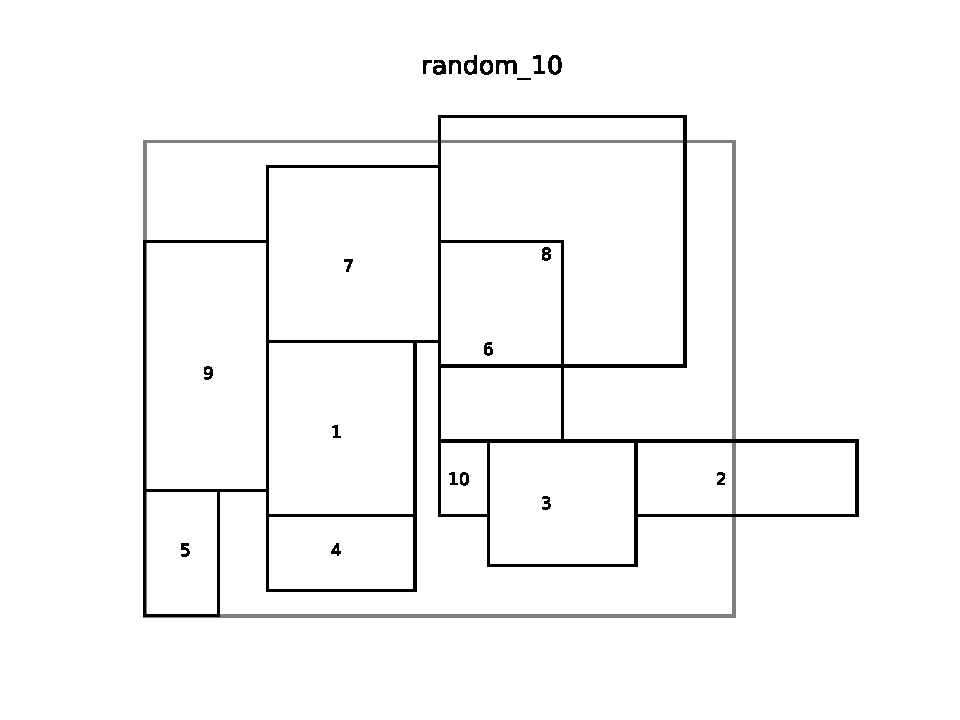
\includegraphics[width=0.9\textwidth]{visualization_random10_brute}\label{subfig:random10-brute}}

    \subfloat[proposed solution]{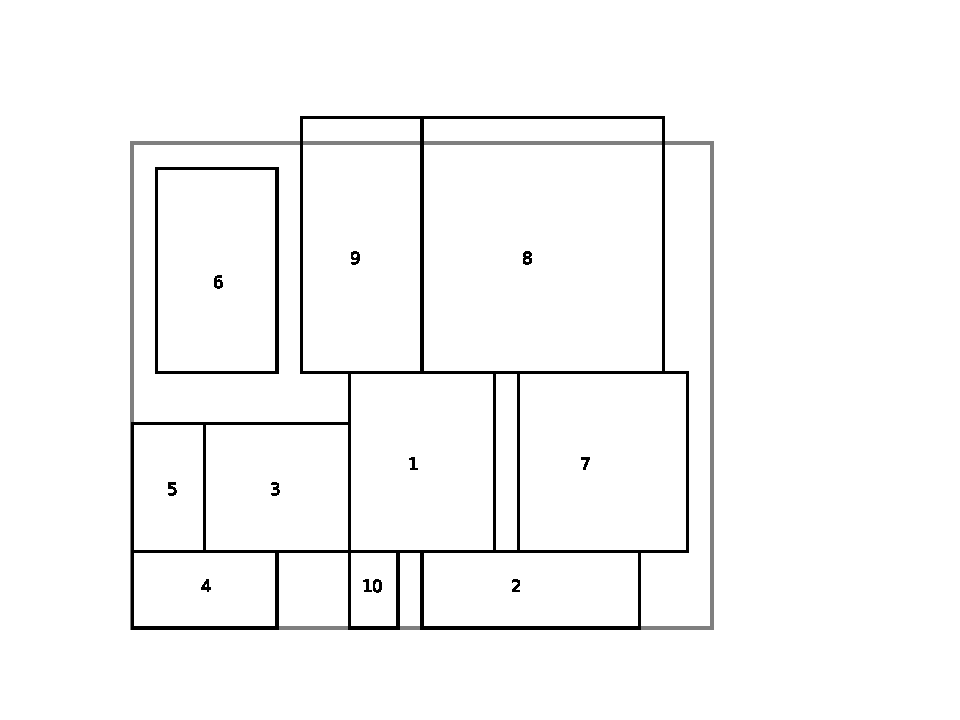
\includegraphics[width=0.9\textwidth]{visualization_random10_ga}\label{subfig:random10-ga}}
    \caption[Random\_10 instance solution visualization for brute-force]
        {Visualization of best result of proposed solution and brute-force for random\_10 instance.}
    \label{fig:visualization-random10}%
\end{figure}
%    \end{landscape}
%    \clearpage% Flush page
%}

%\afterpage{%
%    \clearpage% Flush earlier floats (otherwise order might not be correct)
%    \begin{landscape}% Landscape page
\begin{figure}[h!]
    \centering
    \subfloat[brute-force]{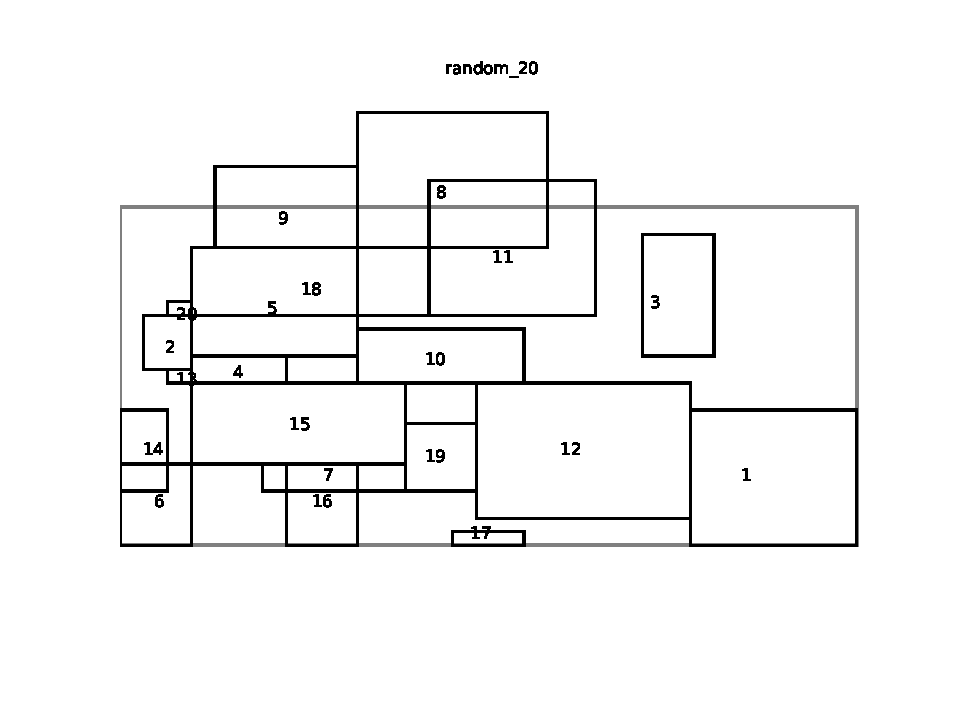
\includegraphics[width=0.8\textwidth]{visualization_random20_brute}\label{subfig:random20-brute}}

    \subfloat[proposed solution]{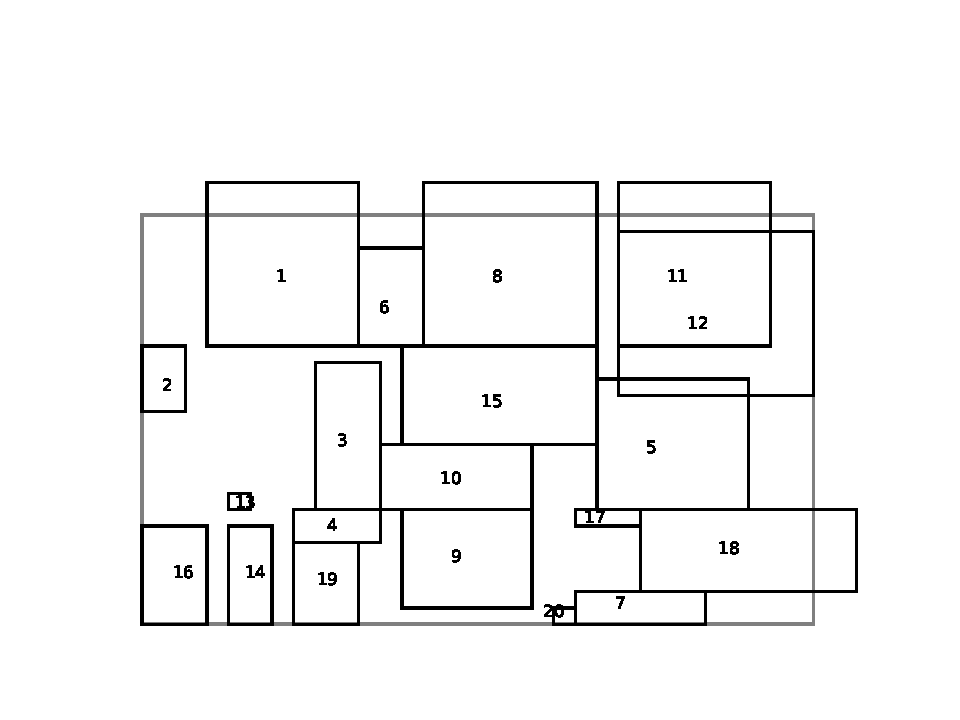
\includegraphics[width=0.8\textwidth]{visualization_random20_ga}\label{subfig:random20-ga}}
    \caption[Random\_10 instance solution visualization for proposed solution]
        {Visualization of best result of proposed solution and brute-force for random\_20 instance.}
    \label{fig:visualization-random20}%
\end{figure}
%    \end{landscape}
\clearpage% Flush page
%}

%\afterpage{%
%    \clearpage% Flush earlier floats (otherwise order might not be correct)
%    \begin{landscape}% Landscape page
\begin{figure}[h!]
    \centering
    \subfloat{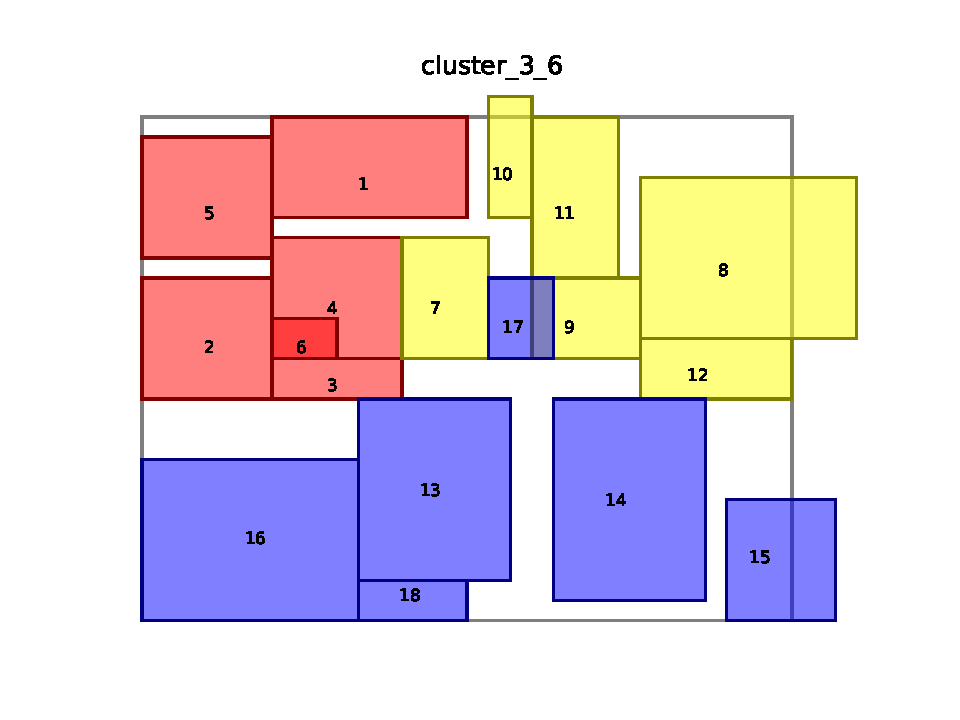
\includegraphics[width=0.8\textwidth]{visualization_cluster_3_6_ga}\label{subfig:cluster-3-6-ga}}

    \subfloat{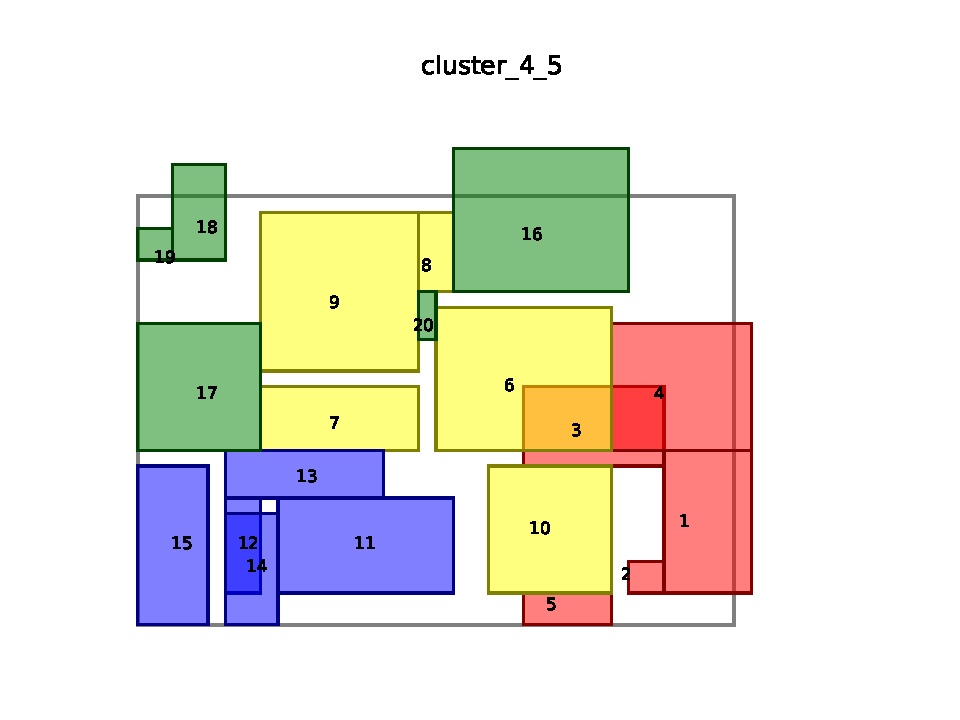
\includegraphics[width=0.8\textwidth]{visualization_cluster_4_5_ga}\label{subfig:cluster-4-5-ga}}
    \caption[Solution visualization of clustering instances for proposed solution]
    {Visualization of the best result of proposed solution for instances cluster\_3\_6 and cluster\_4\_5.}
    \label{fig:visualization-cluster}%
\end{figure}
%    \end{landscape}
%    \clearpage% Flush page
%}

%\afterpage{%
%    \clearpage% Flush earlier floats (otherwise order might not be correct)
%    \begin{landscape}% Landscape page
\begin{figure}[h!]
    \centering
    \subfloat{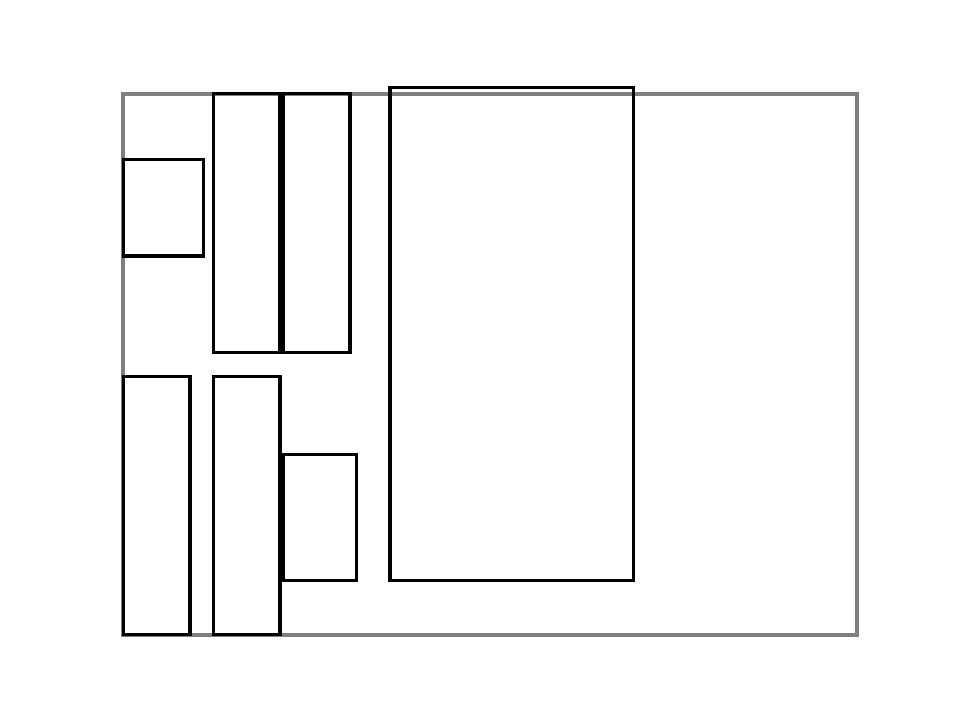
\includegraphics[width=0.8\textwidth]{visualization_london_nationa_gallery_ga}\label{subfig:london-gallery-ga}}
    \caption[London National Gallery solution visualization]
    {Visualization of the London National Gallery wall dataset.}
    \label{fig:visualization-cluster}%
\end{figure}
%    \end{landscape}
%    \clearpage% Flush page
%}

\clearpage% Flush earlier floats (otherwise order might not be correct)
\newpage


\section{Implementation}\label{sec:implementation}

The proposed implementation of a genetic approach is written in Java 11
using a Play Framework v2.8\footnotemark[1], a web framework for Java and Scala.

Implementation behaves like a computation server to which
a user can submit a computation.
Then, the server asynchronously starts the submitted computation and returns an identifier of the computation.
It means that multiple computations can be submitted without blocking the user.
The user can then check the computation state using the returned identifier.

To start the computation server, locate the directory containing a file \verb|build.sbt| in the attached medium (see appendix~\ref{ch:contents-of-the-attached-medium}).
Then, run the following command in that directory (Java~11, SBT\footnotemark[3], and Scala must be installed).

\begin{listing}[h!]
    \begin{cminted}[autogobble,breaklines=true]{shell}
        $ sbt run
    \end{cminted}
    \caption[Starting a computation server]
    {Starting a computation server.}
    \label{lst:sbt-run}
\end{listing}

Command in listing~\ref{lst:sbt-run} uses \verb|sbt|\footnotemark[3] with \verb|run| argument to start the computation server.
By default, the computation server accept requests on \verb|localhost:9000|.
An example of submitting a computation with a predefined instance name to the computation server is in listing~\ref{lst:computation-submission-dataset}.
An example of a successful computation submission response is in listing~\ref{lst:computation-response-success}.

\begin{listing}[h!]
%    \centering
    \begin{cminted}[autogobble,breaklines=true]{json}
    {
        "id":"random_10_9B5F8",
        "outputDirectory":"./out/088_random_10_9B5F8"
    }
    \end{cminted}
    \caption[Successful computation submission response]
    {Successful computation submission response.}
    \label{lst:computation-response-success}
\end{listing}

The computation server also validates input before starting the computation.
For example, if misspelling the instance name, the response by the computation server can be seen in~\ref{lst:computation-response-fail}.

\begin{listing}[h!]
    \centering
    \begin{cminted}[autogobble,breaklines=true]{json}
    {
        "message":"Entity [DatasetDto] with identifier [randomm_10] was not found."
    }
    \end{cminted}
    \caption[Unsuccessful computation submission response]
    {Unsuccessful computation submission response.}
    \label{lst:computation-response-fail}
\end{listing}

Lastly, there is also an option not to specify the instance name in the submission, as seen
in listing~\ref{lst:computation-submission-dataset} where the instance name is random\_10.
In that case, a user has to specify the instance manually in the request – layout width and height,
paintings together with their flow and evaluation function $\pi$ (eq.~\ref{eq:objective}), in the format that is accepted by
mXparser\footnotemark[4].
An example of submission without specifying the instance name is in the appendix in listing~\ref{lst:computation-submission-manual}.

% @formatter:off
\begin{listing}[h!]
\centering
\begin{minted}[autogobble,breaklines=true]{shell}
$ curl --location 'localhost:9000/compute/dataset' \
--header 'Content-Type: application/json' \
--data '{
  "datasetName": "random_10",
  "gaParameters": {
    "maxNumberOfIter": 300,
    "populationSize": 500,
    "maximumWildCardCount": 1,
    "orientationWeights": [
      1,
      1,
      0.5
    ],
    "geneticAlgorithm": "simpleGa",
    "mate": "normalizedProbabilityVectorSum",
    "mutate": "flipOnePartAtRandom",
    "select": "tournament",
    "objective": "simple",
    "evaluator": "ga",
    "placingHeuristics": "corner",
    "populationDivisionCounts": {
      "elite": 0.2,
      "average": 0.6,
      "worst": 0.2,
      "children": 0.3,
      "mutant": 0.2,
      "winner": 0.2,
      "random": 0.1
    },
    "initialPopulationDivisionCounts": {
      "random": 0.7,
      "greedy": 0.3
    }
  },
  "objectiveParameters": {
    "name": "simple",
    "params": {
      "overlappingPenalizationConstant": 30.61,
      "outsideOfAllocatedAreaPenalizationConstant": 30.61
    }
  }
}'
\end{minted}
\cprotect\caption[Example of computation submission with instance name]
{Example of computation submission of random\_10 instance using \verb|curl|\footnotemark[2] to a computation server running on \verb|localhost:9000|.}
\label{lst:computation-submission-dataset}
\end{listing}
% @formatter:on

\footnotetext[1]{\url{https://www.playframework.com/documentation/2.8.x/Home}}
\footnotetext[2]{\url{https://curl.se/}}
\footnotetext[3]{\url{https://www.scala-sbt.org/}}
\footnotetext[4]{\url{https://mathparser.org/}}

